
\documentclass[a4paper,11pt]{article}
\usepackage[utf8]{inputenc}
\usepackage[T1]{fontenc}
\usepackage[frenchb]{babel}

\usepackage{graphicx}
\usepackage{fancyhdr}
\usepackage{geometry}

\usepackage[colorlinks,linkcolor=blue]{hyperref}
\usepackage{amsmath}
\usepackage{amssymb}
\usepackage{mathrsfs}
\usepackage{epsfig}
\usepackage {eurosym}

\usepackage{float}

\geometry{a4paper,tmargin=2cm,bmargin=2cm,lmargin=1.5cm,rmargin=1cm,headheight=2.2cm,headsep=0.5cm,footskip=1cm}
\columnsep=0.6cm

\graphicspath{{images/}} 

\usepackage{listings}
\usepackage{color}
\usepackage{xcolor}

\lstset{columns=flexible,keepspaces=true, breaklines,breakindent=0pt} 


\lstset{language=C++,
basicstyle=\ttfamily\footnotesize,
breaklines, 
keywordstyle=\bfseries\color{blue},
stringstyle=\color{red},
commentstyle=\color{blue!20!black!30!green},
morecomment=[s][\color{black}]{/**}{*/},
numbers=left,
numberstyle=\tiny\color{black},
stepnumber=2,
numbersep=10pt,
tabsize=4,
showspaces=false,
showstringspaces=false}


\fancypagestyle{plain}{
% noms des respo   dans le bas de page                                            
\lfoot{Projet de C++}
\rfoot{M.Morin J.Fourmann}
\renewcommand{\headrulewidth}{0pt}
\fancyhead{}}
% Titre a compl»ter
\title{\textbf{ \huge{Projet de programmation C++}} \\{\Large  Résolution de circuit}}

\author{
\textsc{Jérémie Fourmann} (Promo 2013 - Eléctronique - Enseeiht)\\ %mettre votre nom
\textsc{Maxime Morin} (Promo 2013 - Eléctronique - Enseeiht)\\ %mettre votre nom
%\textsc{ddd dddd} (Promo - departement - respo)     %2 nom
}

\graphicspath{{images/}}

\begin{document}

\pagestyle{plain}

\maketitle
\vspace{1cm}
\renewcommand{\contentsname}{Plan}
\tableofcontents
\vspace{2cm}



\newpage


%Objectif

\section{Objectif}
\section{Organistion du code}
  \subsection{L'objet circuit}
    \begin{figure}[H]
	 \begin{center}
	  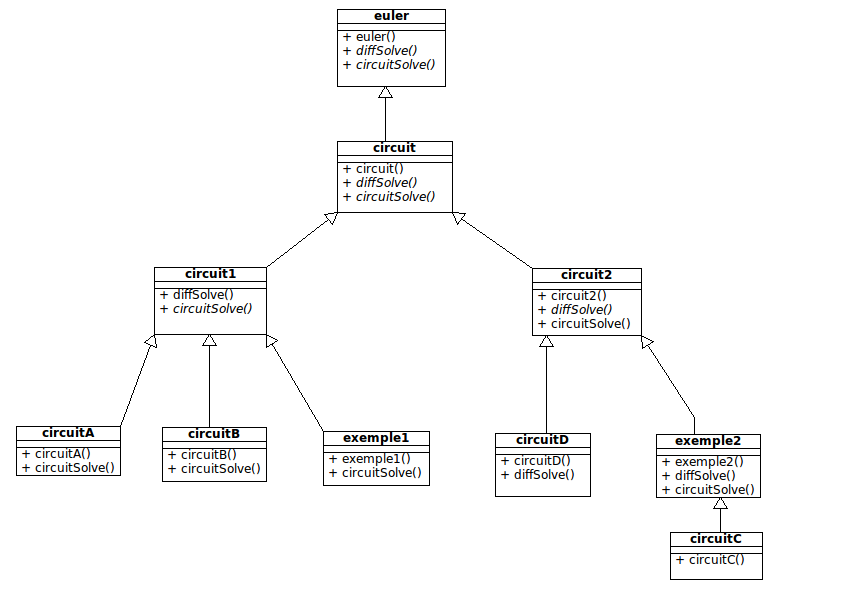
\includegraphics[scale=.7]{circuitDiagram}
	\caption{Hièrarchie de la classe circuit}
	\end{center}
      \end{figure}

  \subsection{L'objet source}
    \begin{figure}[H]
	 \begin{center}
	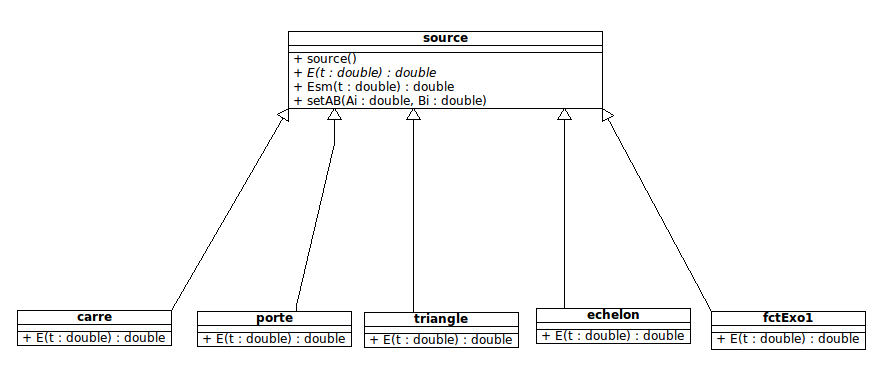
\includegraphics[scale=.7]{sourceDiagram}
	\caption{Hièrarchie de la classe source}
	\end{center}
      \end{figure}
\newpage


\section{Résultats}
  \subsection{Exemple 1}
Résolution de l'équation différentielle du 1\ier ordre :
\begin{equation*}
 \left \{
  \begin{array}{c @{=} l}
    u'(t) & -3\cdot u(t)-3\cdot t
\\
   u(0) & 0
  \end{array}
\right.
\end{equation*} 

La solution exacte étant $u(t)=-1/3\cdot exp(-3t)-1/3$
  \begin{figure}[H]
	 \begin{center}
	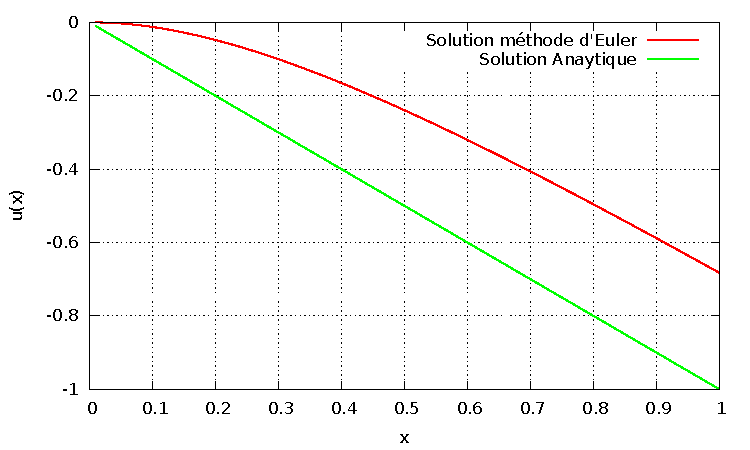
\includegraphics[scale=1]{exemple1}
	\caption{Solution de l'exemple 1}
	\end{center}
      \end{figure}
\subsection{Exemple 2}
Résolution de l'équation différentielle du 1\ier ordre :
\begin{equation*}
 \left \{
  \begin{array}{c @{=} l}
    u''(t) & -\lambda \cdot u(t) 
\\
   u(0) & 0
\\
  u'(0)&1
  \end{array}
\right.
\end{equation*} 

La solution exacte étant $u(t)=sin(t)$

  \begin{figure}[H]
	 \begin{center}
	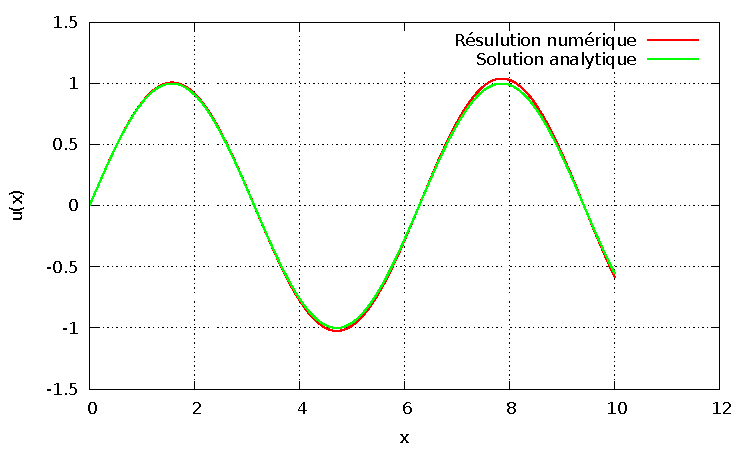
\includegraphics[scale=1]{exemple2}
	\caption{Solution de l'exemple 2}
	\end{center}
      \end{figure}

\newpage


  \subsection{Réponse du CircuitA}
\begin{figure}[h!]
   \begin{minipage}[b]{0.5\linewidth}
      \centering 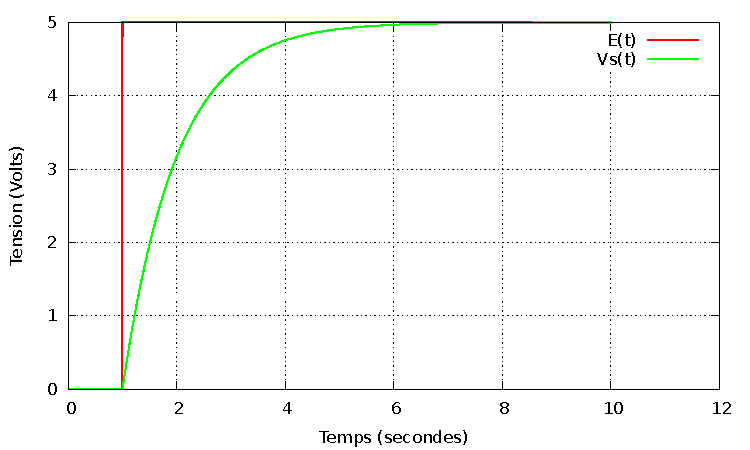
\includegraphics[scale=0.68]{CAechelon.pdf}
   \end{minipage}\hfill
   \begin{minipage}[b]{0.5\linewidth}   
      \centering 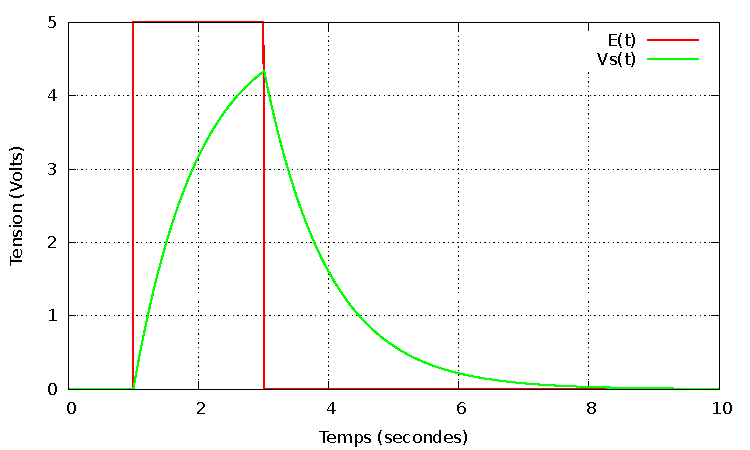
\includegraphics[scale=.68]{CAporte.pdf}
   \end{minipage}\\
    \begin{minipage}[b]{0.5\linewidth}   
      \centering 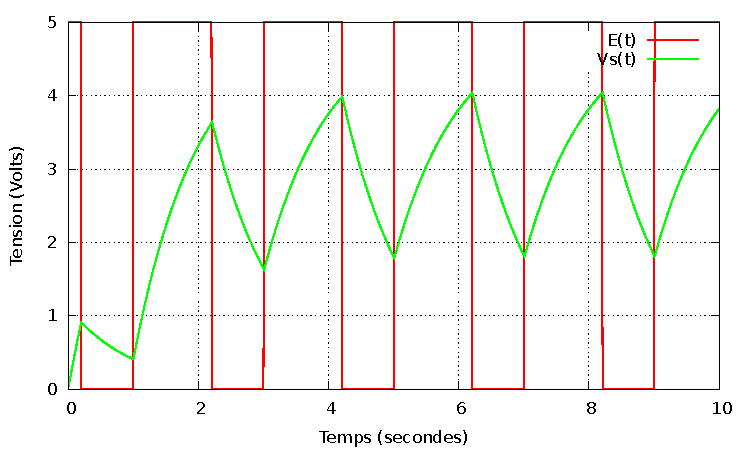
\includegraphics[scale=.68]{CAcarre.pdf}
   \end{minipage}
  \begin{minipage}[b]{0.5\linewidth}   
      \centering 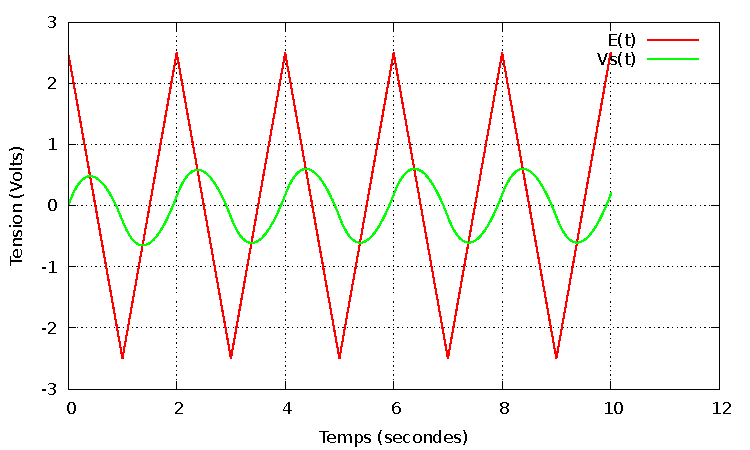
\includegraphics[scale=.68]{CAtriangle.pdf}
   \end{minipage}\\
 \caption{Réponse du circuit A}
\end{figure}

\newpage
  \subsection{Réponse du CircuitB}

  \begin{figure}[h!]
   \begin{minipage}[b]{0.5\linewidth}
      \centering 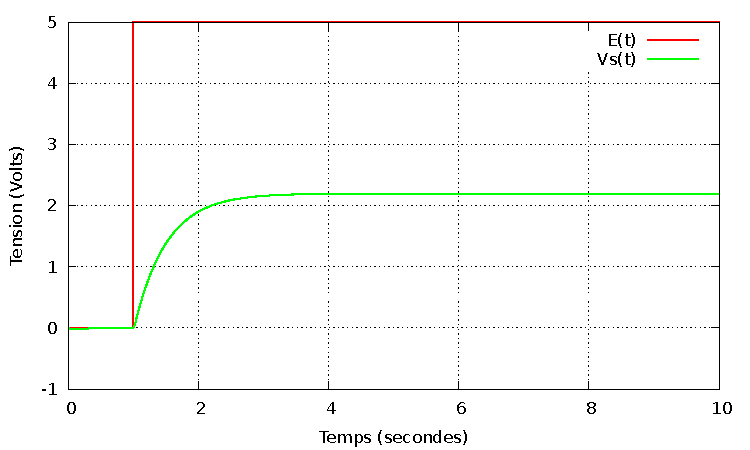
\includegraphics[scale=0.68]{CBechelon.pdf}
   \end{minipage}\hfill
   \begin{minipage}[b]{0.5\linewidth}   
      \centering 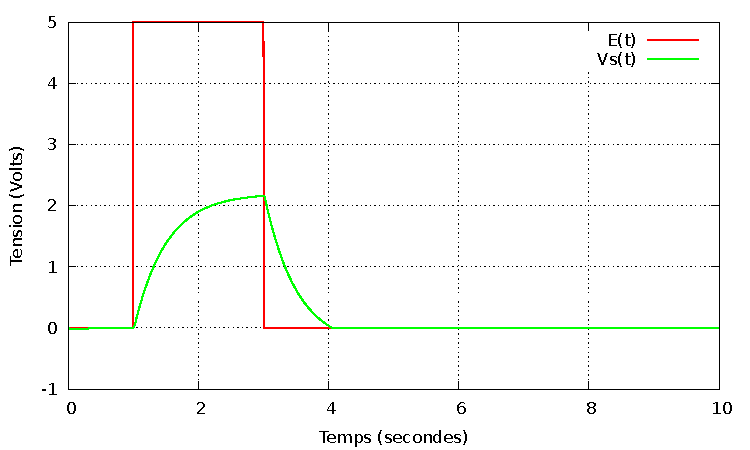
\includegraphics[scale=.68]{CBporte.pdf}
   \end{minipage}\\
    \begin{minipage}[b]{0.5\linewidth}   
      \centering 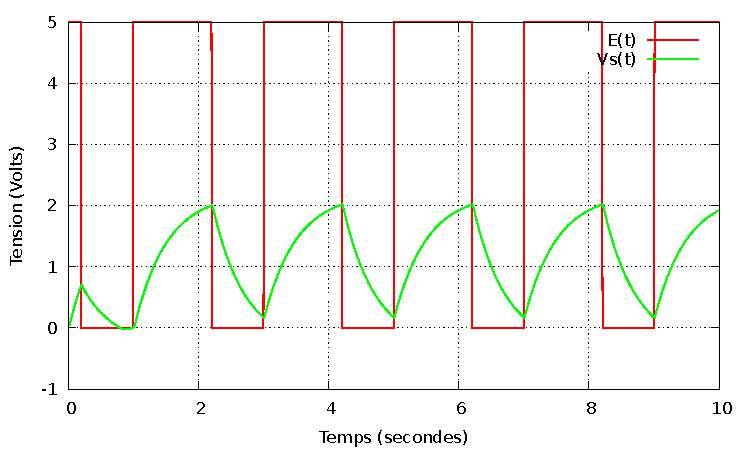
\includegraphics[scale=.68]{CBcarre.pdf}
   \end{minipage}
  \begin{minipage}[b]{0.5\linewidth}   
      \centering 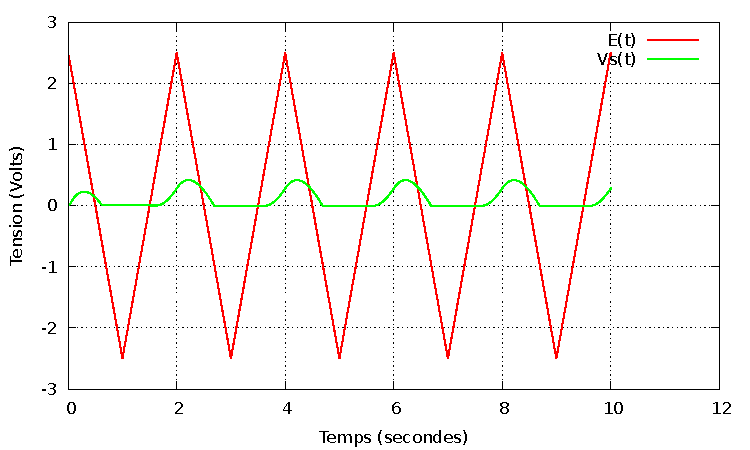
\includegraphics[scale=.68]{CBtriangle.pdf}
   \end{minipage}\\
 \caption{ Réponse du circuit B}
\end{figure}
\newpage
  \subsection{Réponse du CircuitC}

  \begin{figure}[h!]
   \begin{minipage}[b]{0.5\linewidth}
      \centering 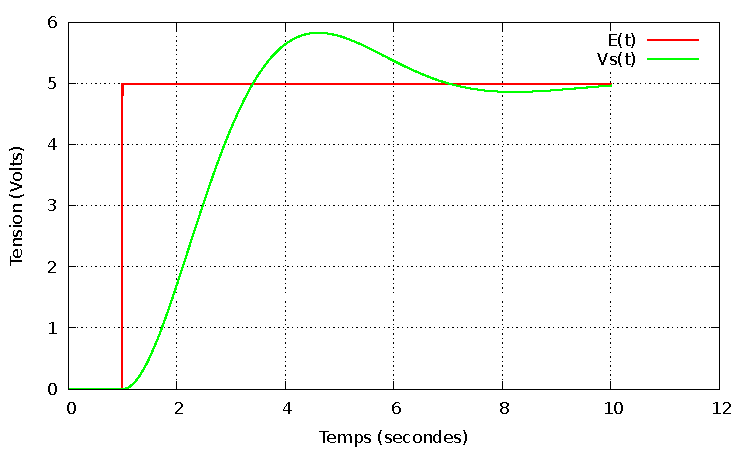
\includegraphics[scale=0.68]{CCechelon.pdf}
   \end{minipage}\hfill
   \begin{minipage}[b]{0.5\linewidth}   
      \centering 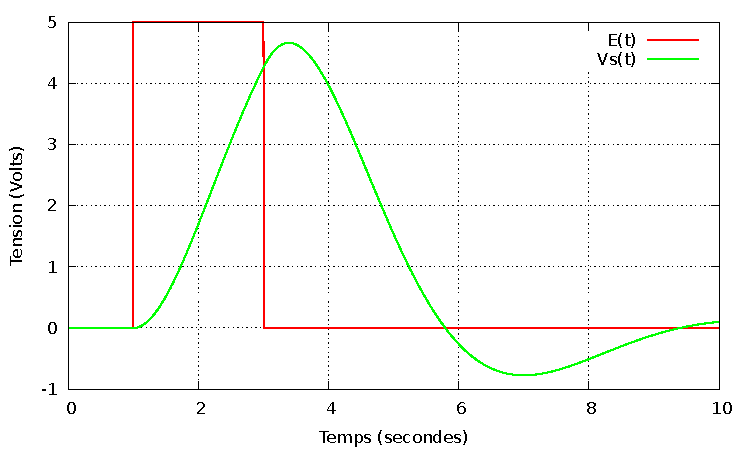
\includegraphics[scale=.68]{CCporte.pdf}
   \end{minipage}\\
    \begin{minipage}[b]{0.5\linewidth}   
      \centering 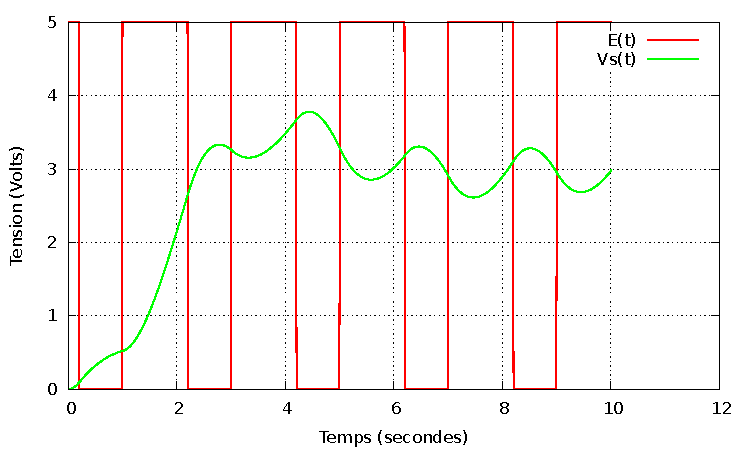
\includegraphics[scale=.68]{CCcarre.pdf}
   \end{minipage}
  \begin{minipage}[b]{0.5\linewidth}   
      \centering 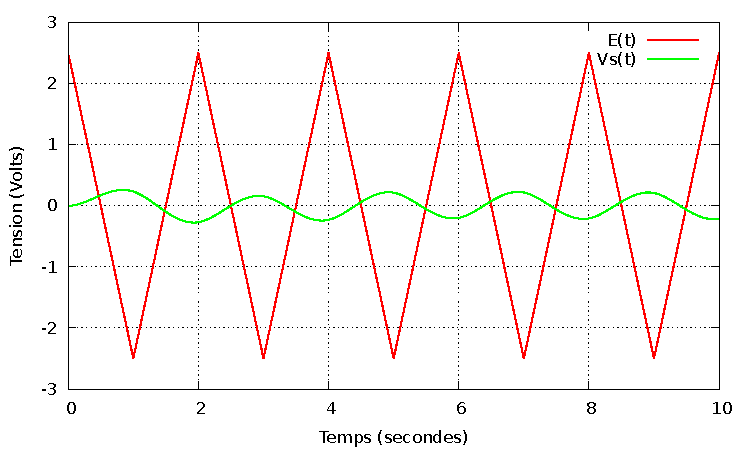
\includegraphics[scale=.68]{CCtriangle.pdf}
   \end{minipage}\\
 \caption{Réponse du circuit C}
\end{figure}

\newpage
  \subsection{Réponse du CircuitD}

\begin{figure}[h!]
   \begin{minipage}[b]{0.5\linewidth}
      \centering 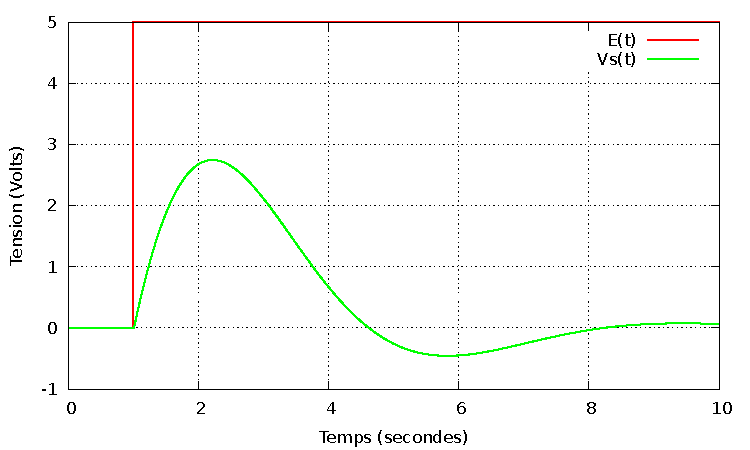
\includegraphics[scale=0.68]{CDechelon.pdf}
   \end{minipage}\hfill
   \begin{minipage}[b]{0.5\linewidth}   
      \centering 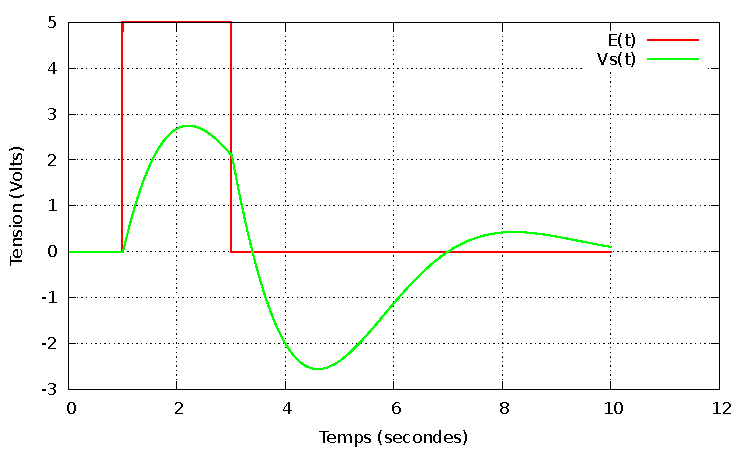
\includegraphics[scale=.68]{CDporte.pdf}
   \end{minipage}\\
    \begin{minipage}[b]{0.5\linewidth}   
      \centering 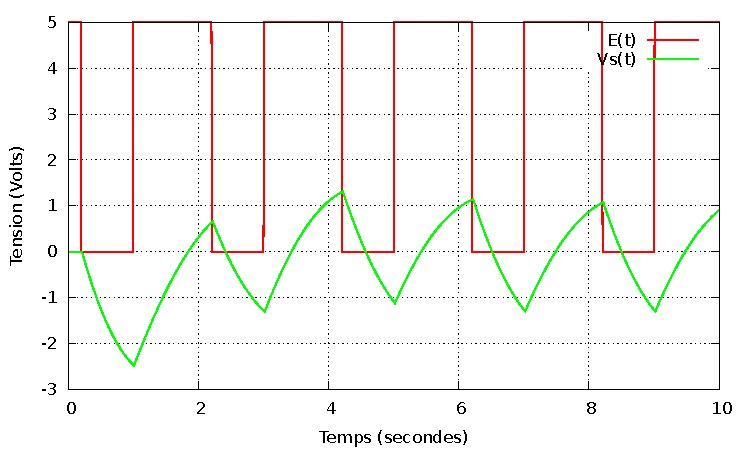
\includegraphics[scale=.68]{CDcarre.pdf}
   \end{minipage}
  \begin{minipage}[b]{0.5\linewidth}   
      \centering 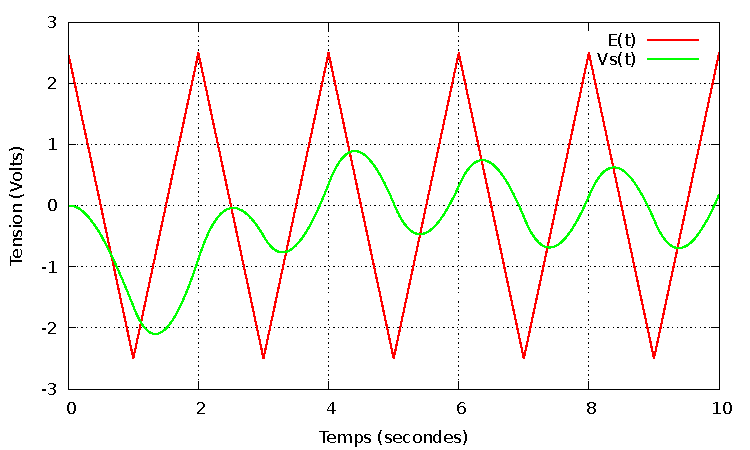
\includegraphics[scale=.68]{CDtriangle.pdf}
   \end{minipage}\\
 \caption{Réponse du circuit D}
\end{figure}




  \newpage
  \appendix
  
  \section{main.cpp}
    \lstinputlisting{../main.cpp}
    \newpage
  \section{circuits.h}
    \lstinputlisting{../circuits.h}
    \newpage
  \section{circuits.cpp}
    \lstinputlisting{../circuits.cpp}
    \newpage
   \section{sources.h}
    \lstinputlisting{../sources.h}
    \newpage
   \section{sources.cpp}
    \lstinputlisting{../sources.cpp}
    \newpage

\end{document}
